\section{Discusión}

Lo primero que queremos destacar es todo el trabajo adicional que requiere el
procesamiento con \textbf{SIMD}. Como vimos en varios casos se abrieron múltiples
posibilidades, no quedando claro a veces cuál es la más conveniente.

En numerosas ocasiones nos topamos con problemas; por ejemplo, a veces parecen no
alcanzarnos los registros; o en otros casos parece que la falta de una instrucción
en el set nos obliga a hacer más cuentas o movimientos de los necesarios.

Es notorio también que en esta arquitectura, pequeños cambios en lo que se quiere
lograr pueden repercutir en el algoritmo de manera muy fuerte, ya que los datos al
estar empaquetados de alguna manera están ``atados''. Por ejemplo, si a las matrices
de 3x3 les quisiéramos poner un 1 en la posición central (aunque esto no tenga
mucho sentido para la detección de bordes) el algoritmo debería transformarse
completamente, ya que los registros se van a agotar y la forma de acomodar los 
valores no va a poder ser la misma.

Otra cuestión que notamos es que haciendo este tipo de códigos, cuyo diseño se basa
fuertemente en la eficiencia, uno corre el riesgo de querer ir demasiado lejos; es
decir, uno empieza a tratar de sacar el máximo jugo a cada operación no conformándose
nunca.

En este aspecto creemos que es importante enfocarse en la optimización ``a gran
escala'' (es decir cómo diseñar las cosas para operar aprovechando la paralelización)
y no preocuparse tanto por hacer ``la mímina cantidad de operaciones''. Lo que queremos
decir es que, quizás por querer evitar un par de operaciones, se puede caer en complicaciones
importantes, cuando en realidad el grueso del trabajo ya está paralelizado y es 
terriblemente eficiente.

\subsection{Comparación entre operadores SIMD}

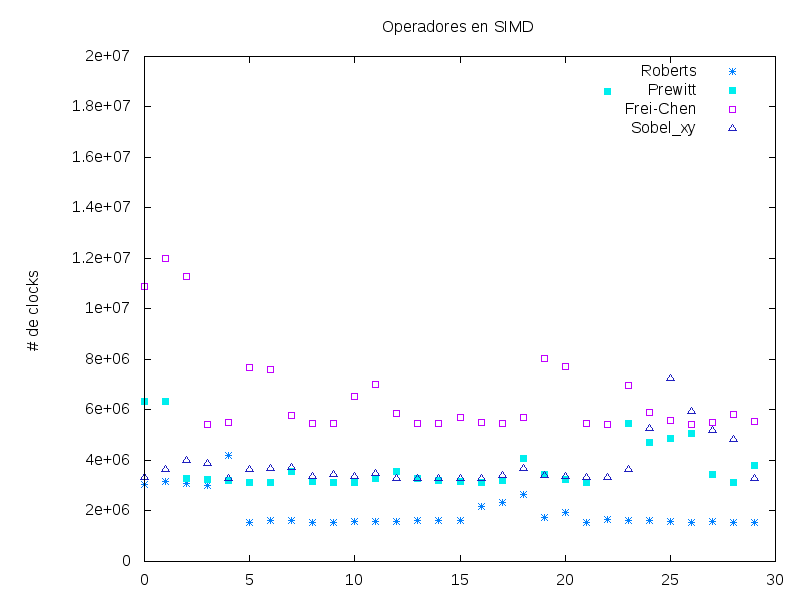
\includegraphics[scale=0.5]{../resultados/operadores.png}

Como se ve en este primer gráfico, la implementación más veloz es la de Roberts.
Esto por supuesto se explica por la simplicidad de ese operador, sobre lo que
hablamos anteriormente. En el otro extremo, la que más tiempo toma es la implementación
de Frei-chen, lo que se debe (al menos en parte) a que opera en punto flotante,
donde todas las operaciones son por naturaleza más costosas.

En ese sentido habríamos esperado encontrarnos con más diferencia aún. Nos parece
notable que el hardware especializado permita con punto flotante hacer cálculos no
mucho más ineficientemente que con enteros.

\subsection{SIMD vs. GPR}

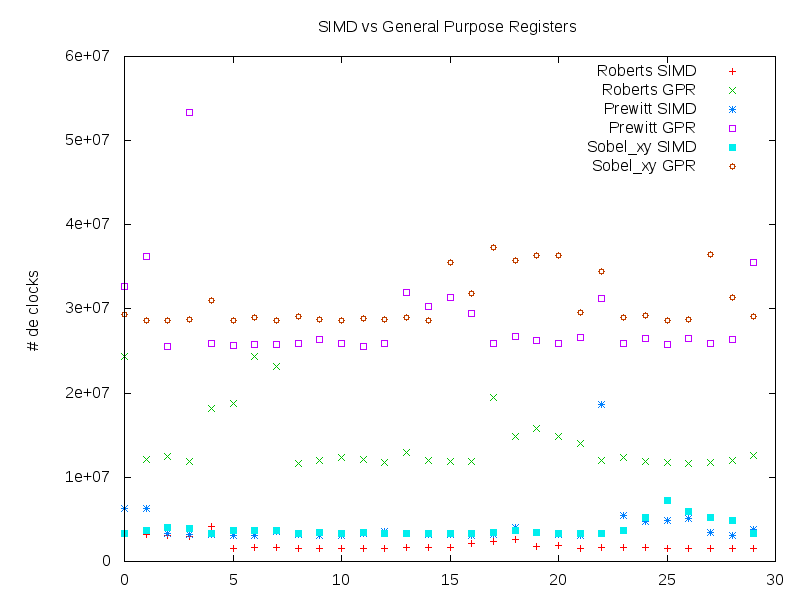
\includegraphics[scale=0.5]{../resultados/simd.png}

Como vemos aquí el procesamiento \textbf{SIMD} realmente es \textbf{otra cosa}.
Las implementaciones que logramos son algo así como 10 veces más eficientes que
las anteriores (¡que ya de por sí corrían en un parpadeo!).

Hacer este tipo de funciones con estas tecnologías realmente vale la pena, pues,
pese al esfuerzo adicional mencionado, finalmente se logró un resultado equivalente
de manera relativamente sencilla, y con un enorme beneficio en relación a la eficiencia.
Además, los procesadores actuales de uso general contienen siempre estas extensiones,
por lo que la portabilidad en la práctica no suele ser un problema.

\pagebreak
\subsection{SIMD vs. OpenCV}

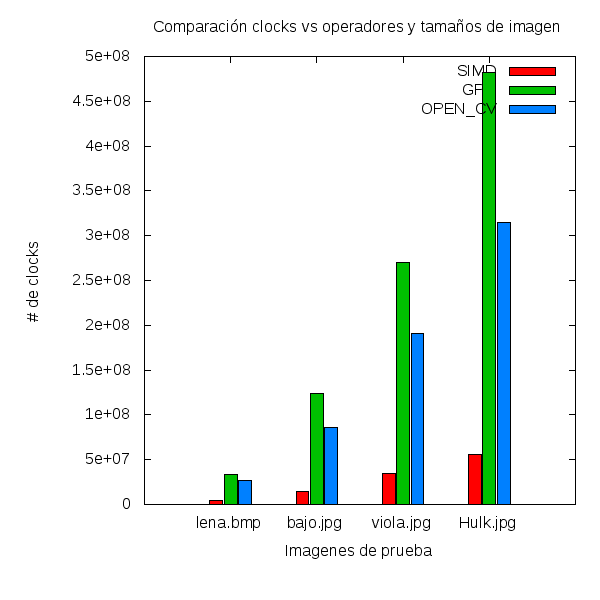
\includegraphics[scale=0.5]{../resultados/graf3.png}

En este último gráfico en el que comparamos la eficiencia de las nuevas implementaciones
de Sobel contra las de \textbf{OpenCV}, podemos observar que se superó el rendimiento de esa
biblioteca. Esto parecería indicar que las implementaciones de \textbf{OpenCV} no usan
XMM sino los registros de propósito general.

Las imágenes de este gráfico son todas ``múltiplos'' en tamaño de \texttt{lena.bmp} en el siguiente sentido: \texttt{bajo.jpg} tiene exactamente el doble de pixeles (1024x1024), \texttt{viola.jpg} tiene 3 $\times$ ``lena'' (1536x1536) y, por último, \texttt{hulk.jpg} que es 4 veces ``lena'' (2048x2048). 




